\Chapter{Hatékonyságnövelő módszerek}

A témám kifejtése előtt érdemesnek tartom átnézni azon módszereket, amelyek hozzájárulnak a hatékony időbeosztás megvalósításához, illetve a már meglévő alkalmazásokat, hogy azok milyen funkciókat látnak el. De mit is takar ez az egész időgazdálkodás pontosan, és miért van erre szükség?

Az időgazdálkodás egy lehetséges definíciója a következő: "Az időgazdálkodás a rendelkezésünkre álló idő felhasználására vonatkozó döntések meghozatala, a legfontosabb teendőink elvégzéséhez szükséges idő biztosítása, továbbá a kapcsolatos információk és iratok kezelése, valamint rendelkezésre állásuk biztosítása." \cite{alapok}.

Az emberek az idővel kapcsolatban mindig két tévhitben élnek. Egyrészt abban, hogy egyszer a jövőben több idejük lesz, másrészt pedig, hogy időt tudnak megtakarítani. Időt azonban nem lehet megtakarítani, hiszen az ugyanolyan ütemben telik el semmittevés során is, mintha sok dolgot végeznénk el. Amit tehetünk az az, hogy a rendelkezésre álló időt jól kihasználjuk és hasznos tevékenységekkel töltjük el, ezáltal pedig produktívabbak leszünk \cite{hatekonyido}.

Brian Tracy a \textit{Személyes hatékonyság} című könyvében pedig tökéletesen kifejtette miért jó az időgazdálkodás, és az, ha produktívak vagyunk:
"Számos tanulmány kimutatta, hogy a legjobban megfizetett és a ranglétrán leggyorsabban emelkedő emberek mind-mind rendelkeznek egy tulajdonsággal, amit úgy hívnak, hogy "cselekvésorientáltság". Minden cselekvésüket áthatja ez a szemlélet. A sikeres és hatékony emberek azok, akik mindig rögtön a fontos feladatokkal kezdenek foglalkozni, és addig nem hagyják ezt abba, amíg be nem fejezték az adott feladatot." \cite{brian}.

Megállapíthatjuk tehát, hogy életünkben jelentős előnyei vannak időnk megfelelő menedzselésének, mint például:
\begin{itemize}
\item a nagyobb produktivitás és hatékonyság elérése,
\item jobb szakmai hírnév,
\item kevesebb stressz,
\item nagyobb valószínűség az előrelépésre,
\item nagyobb valószínűség az élet- és karriercélok elérésére,
\item a mindennapi kötelezettségek könnyebb összeegyeztetése \cite{mindtools}.
\end{itemize}

\Section{Hatékonyságnövelő módszerek}

Nem újkeletű téma annak kutatása, hogy hogyan lehet több időt nyerni magunknak; a régi időkben is sokakat foglalkoztatott már ez a kérdés. Számtalan módszert dolgoztak ki, megannyi technikáról olvashatunk ezzel a témakörrel kapcsolatban. A következőkben ezek közül tekintek át néhány ismertebb megoldást.

\SubSection{Eisenhower módszer}

Az egyik legismertebb technikát, az \textit{Eisenhower módszer}t -- más néven prioritás mátrixot -- Dwight D. Eisenhower, az Egyesült Államok 34. elnöke dolgozta ki. Mielőtt elnökké vált, tábornokként és parancsnokként is szolgált a második világháború alatt, ahol minden nap kemény döntéseket kellett hoznia arról, hogy a sok feladat közül melyikre kell összpontosítania. Ez végül arra késztette, hogy feltalálja a világhírű \textit{Eisenhower-elv}et, amely ma sürgősség és fontosság alapján segít teendőinket kezelni.

\begin{figure}[h]
	\centering
	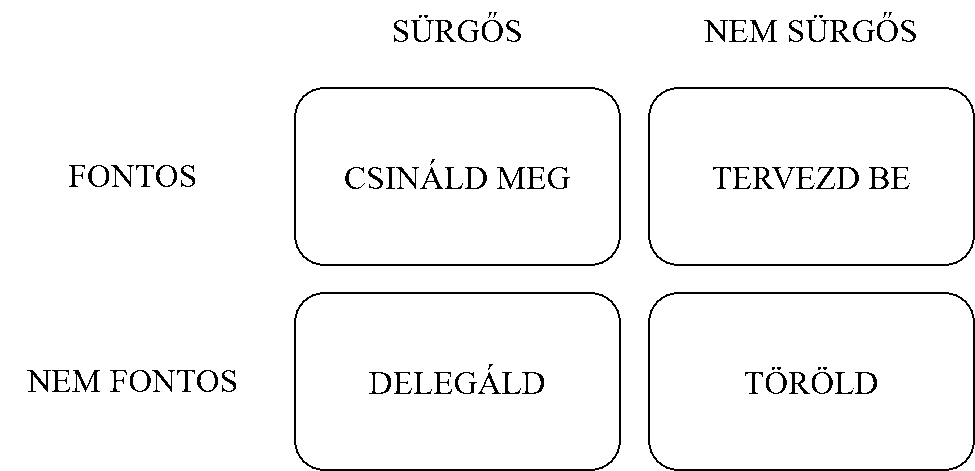
\includegraphics[scale=0.7]{images/eisenhower.png}
	\caption{Az Eisenhower mátrix}
	\label{fig:eisenhower}
\end{figure}

Négy csoportot kapunk így, amelyekhez külön utasítások társulnak (\ref{fig:eisenhower}. ábra).

\begin{itemize}
\item Az első negyed a „Csináld meg” kategória, amely azokat a feladatokat tartalmazza, amelyek fontosak és amiket szükséges még aznap, vagy legkésőbb másnap megcsinálni.
\item A második negyed a „Tervezd be” kategória. Ide tartoznak azok a feladatok, amelyek fontosak, viszont kevésbé sürgősek. Ezeket célszerű betáblázni a közeljövőbe.
\item A harmadik negyed azon feladatoknak van fenntartva, amelyeket delegálhatunk, mivel számunkra kevésbé fontosak, de még mindig elég sürgősek. Érdemes nyomon követni ezeket a megbízásokat, hogy később megbizonyosodjunk előrehaladásukról.
\item A negyedik és egyben az utolsó negyed a „Töröld” kategória. Ide tartoznak, azok a feladatok, amelyekkel egyáltalán nem kéne foglalkozni. Ilyenek lehetnek a rossz szokások, például a felesleges internetezéssel való időtöltés \cite{matrix}.
\end{itemize}
 
\SubSection{Pomodoro technika}

A Pomodoro technika lényege, hogy miután kiválasztottunk egy feladatot, amin dolgozni szeretnénk, 25 percig csak arra fókuszálunk. Miután letelt ez az időtartam, 5 perc szünetet tartunk, majd kezdődhet a következő intervallum. 4 periódus után pedig egy hosszabb, 20-30 perces pihenőidő ajánlott, mielőtt újra munkába lendülnénk \cite{cirillo2006pomodoro}.

A Pomodoro sokak körében ismert és használt hatékonyságnövelő módszer, amely segít abban, hogy egy adott feladatra koncentráljunk és azt teljesítsük, viszont a szakdolgozatomban több feladat időbeli ütemezése a cél egy adott időkereten belül, így nem tartom célszerűnek erre a technikára több figyelmet fordítani.

\SubSection{GTD}

A \textit{Getting Things Done} (röviden GTD) módszerét David Allen tanácsadó ismerteti \textit{Hatékonyságnövelés stresszmentesen} című könyvében. A munkafolyamat 5 lépésből áll, melyek a következők:
\begin{enumerate}
\item Rögzítés,
\item Tisztázás,
\item Rendszerezés,
\item Reflektálás,
\item Cselekvés.
\end{enumerate}

A rögzítés lépése arra szolgál, hogy ne kelljen mindent állandóan észben tartanunk. Ennélfogva rögzítenünk kell valamilyen módon -- akár írásos, akár digitális formában -- minden feladatot, amelyet meg kell csinálnunk.

A tisztázás lépését \aref{fig:tisztazas}. ábra szemlélteti.

\begin{figure}[h]
	\centering
	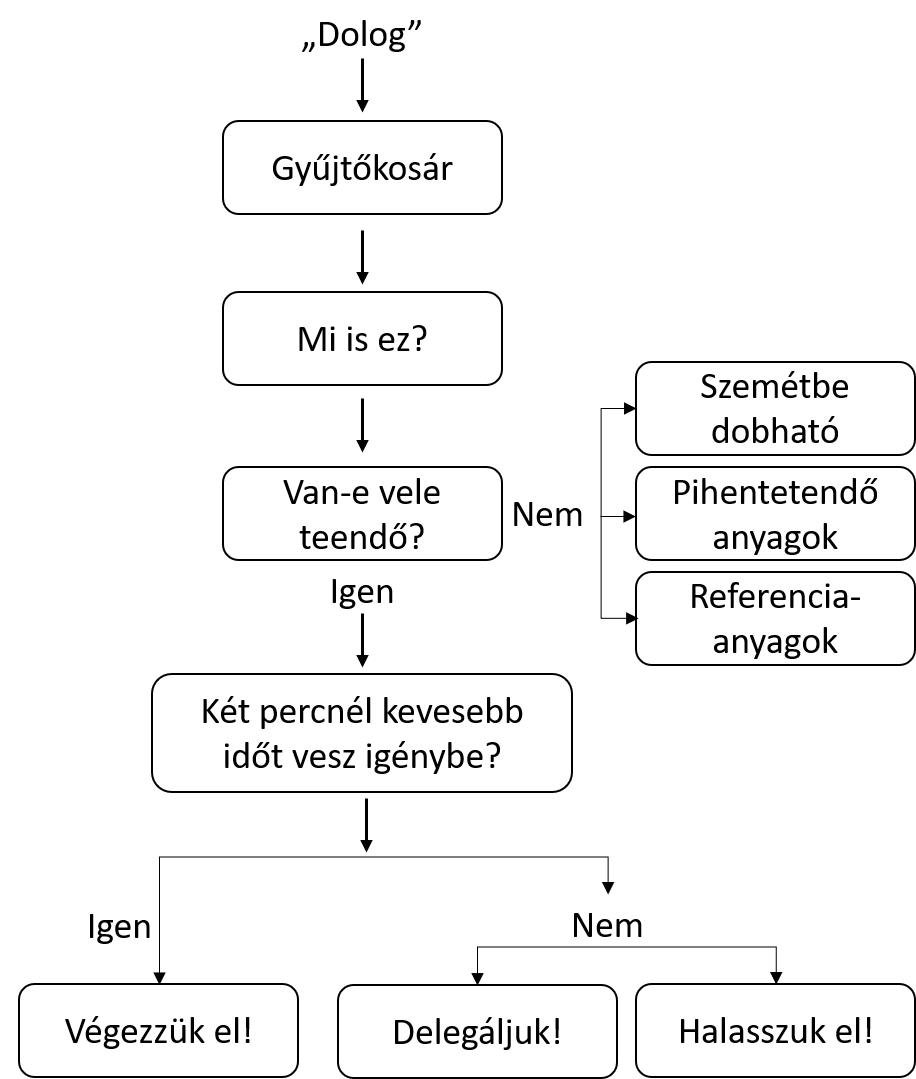
\includegraphics[scale=0.6]{images/tisztazas.png}
	\caption{A tisztázás lépései}
	\label{fig:tisztazas}
\end{figure}

Ha van egy adott „dolog”, elsősorban meg kell győződnünk arról, hogy van-e vele valami teendőnk. Ha nincsen, akkor eldöntjük, hogy szemétbe dobható-e, később lesz-e vele valami teendőnk, vagy pedig potenciálisan hasznos információt tartalmaz, amely később még szükséges lehet számunkra.

Amennyiben az adott dologgal kapcsolatban van teendőnk, akkor három lehetőség közül választhatunk.
\begin{itemize}
\item Ha egy teendő két percnél kevesebb időt vesz igénybe, célszerű abban a pillanatban elvégeznünk, amelyben döntünk róla.
\item Ha tovább tart, mint két perc, fel kell tennünk magunkban a kérdést miszerint mi vagyunk-e a legalkalmasabbak erre a feladatra, és ha nem, akkor érdemes egy megfelelő emberre átruházni a feladatot.
\item Ha két percnél hosszabb időt vesz igénybe az adott tevékenység, és mi vagyunk rá a legalkalmasabbak, akkor vagy későbbre halasztjuk vagy a következő lépésre ugrunk a munkafolyamatunkban, tehát amint lehet megcsináljuk.
\end{itemize}

Érdemes megfigyelni, hogy alapjaiban véve az Eisenhower módszerhez hasonló megközelítések merülnek fel itt is. Elvégre megjelenik a delegálás, továbbá annak mérlegelése, hogy valamit betervezzünk-e a későbbiekre, vagy kezdjünk el vele az adott pillanatban foglalkozni.

A rendszerezés lépése a dolgaink feldolgozásában és értékelésében segítenek, hiszen fontos, hogy fizikai formában is tároljuk és láthatóvá tegyük a különböző kategóriákba tartozó elemeket.

A reflektálás lényege, hogy átnézzük és aktualizáljuk hetente a listáinkat, hogy azok folyamatosan rendszerezve legyenek, naprakészek maradjanak, könnyebben tudjunk fókuszban maradni.

A cselekvés pedig arról szól, hogy a felállított rendszert bizalommal használjuk, mivel minden döntésünk intuitív \cite{gtd}.

\SubSection{Kétperces technika}
\label{sec:twominutes}

A kétperces technika különállóan is megállja a helyét a hatékonyságnövelő módszerek között, de amint az előbb megfigyelhettük, a GTD módszerben is hasznosították ezt a stratégiát, megerősítve ezzel azt, hogy a rövidebb idő alatt elvégezhető feladatok sokat nyomnak a latba a prioritási tényező mellett.

\SubSection{Ivy Lee}

Ivy Lee módszere egészen 1918-ig nyúlik vissza, amikor is Charles M. Schwab a cége hatékonyságának növelése érdekében alkalmazta őt. A 100 éves stratégia azon alapszik, hogy minden este leírjuk a 6 legfontosabb feladatot, amit másnap el szeretnénk végezni és prioritásuk szerint megjelöljük őket. Másnap a feladatoknak egyesével kezdünk neki; amikor végeztünk eggyel, akkor lépünk a következőre. A stratégia azért működőképes, mert csökkenti az egyszerre túl sok döntés meghozatalával járó nehézségeket és az időspóroláson kívül segít céljaink priorizálásában is \cite{ivylee}.

Nyilvánvalóan beszélhetnénk még olyan alternatívákról/opciókról, mint a kanban rendszer, a Zen To Done, a POSEC, Pareto 80/20-as szabálya, mindazonáltal egyértelműen megállapítható, hogy a két alappillér a prioritás és az idő értéke, melyek jelentős szerepet játszanak a minél hatékonyabb időbeosztás elérésében.

\Section{Hatékonyságnövelő alkalmazások}

A különböző módszerek mellett nem szabad elfeledkeznünk arról, hogy tennivalóink rendszerezésének megkönnyítésére mára már számos alkalmazás  létrejött. Ezek többsége azért hasznos, mert nem papír alapú, így könnyen tervezhető, átlátható és többségüket magunknál hordozhatjuk egész nap. Ezek közül a legismertebbeket vesszük most sorra, hogy megállapítsuk, hogy a mai applikációk milyen mértékben alkalmazzák az előző pontokban említett módszereket, és hogyan járulnak hozzá a rendszerezéshez és hatékonyságnöveléshez.

\SubSection{Evernote}

Vitathatatlan, hogy napjaink egyik legismertebb hatékonyságnövelő alkalmazása az Evernote. Alapjáraton ez az alkalmazás nem kifejezetten csak to-do listák készítésére használatos, de megoldható vele feladatlisták létrehozása, amelyekhez emlékeztetőket tudunk beállítani és a jelölőnégyzetek lehetőséget adnak az elvégzett teendők megjelölésére.

Hátránya, hogy naptár funkciót nem tartalmaz, és a szinkronizálás megoldása (pl. más naptár alkalmazásokkal) se egy egyszerű művelet, viszont lehetőségünk van különböző sablonok felhasználására, amik között ma már találunk napi, heti, havi és éves szintű tervező sablonokat, de akár szokáskövetőt is. Érdemes lehet megemlíteni, hogy a sablonok között találunk GTD kategóriát is.

\SubSection{Trello}

A Trello egy olyan alkalmazás, amely kimondottan a személyes hatékonyság és az időgazdálkodás javítására szolgál. Különböző úgynevezett Trello-táblákat hozhatunk létre, kiválasztva a számunkra legmegfelelőbb módszert céljaink elérésére.

Az alkalmazásban található személyes termelékenységi rendszer egy heti feladatrendszerező megoldás, amely segít a feladatlisták kézbentartásában és teendőink áttekintésében.

A táblák közül választhatunk olyat is, amelyik kifejezetten az Eisenhower mátrix módszerének megvalósításához nyújt grafikus felülelet. Ennek segítségével tehát minden feladat és teendő fontosság és sürgősség alapján priorizálható. Ez a tábla segít a hosszú távú célokon tartani a fókuszt, kiszűrve a figyelmet elterelő feladatokat, amelyek miatt nincs idő a lényegi munkára.

A heti felülvizsgálati folyamat tábláján feladatainkat a \textit{Teendők}, a \textit{Folyamatban} és a \textit{Kész} listák használatával tervezzük meg. A heti áttekintő ellenőrzőlisták alkalmazásával könnyedén követhetők a legfontosabb célok és az elért eredmények. Ennek a folyamatnak az alkalmazását David Allen, a GTD módszer megalkotója is ajánlja \cite{trello}.

\SubSection{Google Calendar és Google Keep}

A Google Naptár egy általam is használt és kedvelt alkalmazás. Lehetőségünk adódik akár napi, heti vagy havi nézetben áttekinteni eseményeinket és teendőinket. Adott időpontra vagy egész napra vonatkozóan adhatjuk meg az eseményeket, színjelöléseket használhatunk, és úgynevezett saját naptárakat is alkothatunk, ha egy külön projekthez szeretnénk eseményeket rendelni. Ezeket a naptárakat láthatóvá és nem láthatóvá tehetjük, így külön csoportokban jól áttekinthetővé válik minden esemény. Emlékeztetőket és feladatokat lehet létrehozni, az emlékeztetőknél beállítható az ismétlődés naponta, havonta vagy évente, a feladatokhoz pedig megjegyzéseket csatolhatunk.

A Google másik széles körben ismert alkalmazása a Google Keep. Jegyzetek és listák létrehozására alkalmas, emlékeztetőket állíthatunk be, valamint csoportos hozzáférést is engedélyezhetünk egy-egy jegyzethez. Képeket, rajzokat csatolhatunk, színjelölést használhatunk és a gondolataink lediktálására is lehetőség van.

\SubSection{Todoist}

A Todoist rendszere önmagában is működőképes, de összeköthető az Evernote-tal, a Trello-val, a Google Calendar-ral és egyéb programokkal is. Funkciói közé tartozik a projektek létrehozása, amikhez feladatokat társíthatunk, projektekbe ágyazott projekteket hozhatunk létre, ha több szálon futó munkáról van szó, illetve határidőket és emlékeztetőket állíthatunk be. Természetesen adhatunk meg prioritást és a színkódolás is megjelenik. Az alkalmazást gyakran használják a GTD elveire építve \cite{todoist}.

\SubSection{Microsoft To-do}

A Microsoft To-do segít abban, hogy a különböző tevékenységeket egy helyen vezessük. A szerteágazó feladatok rendszerezésére külön listákat alkothatunk, és ezeket meg tudjuk osztani akár családtagokkal, akár csapattagokkal. Ütemterveket tudunk készíteni, feladatokat kiosztani egy-egy csapattagnak, így nyomonkövetve a tevékenységek folyamatának alakulását \cite{todo}.

\SubSection{Funkciók összehasonlítása}

Az alkalmazások funkcióit \aref{tab:minta}. táblázat foglalja össze.

\begin{table}[h]
	\centering
	\caption{Az alkalmazások funkciói}
	\vskip 3mm
	\label{tab:minta}
	\tabcolsep=0.1cm
	\begin{tabular}{|l|c|c|c|c|c|}
		\hline
		 & Evernote & Trello & Google C.és Keep & Todoist & MS To-do \\
		\hline
		to-do lista készítése & x & x & x & x & x \\
		\hline
		emlékeztető beállítása &x & x & x & x & x \\
		\hline
		színjelölés használata &  & x & x & x &   \\
		\hline
		sémák használata & x & x &   & x &   \\
		\hline
		hat.növ. módszerre (is) épül & x & x &   & x &   \\
		\hline
		megosztás másokkal & x & x & x & x & x \\
		\hline
		feladatok optimalizálása &  &   &   &   &   \\
		\hline
	\end{tabular}
\end{table}

Megfigyelhető, hogy az alkalmazások egy része vagy egy adott hatékonyságnövelő módszerre épül, vagy lehetőségünk van bizonyos szinten megvalósítani, felhasználni bennük valamelyiket. A fenti áttekintésből látható az is, hogy funkciók tárháza áll rendelkezésre a rendszerezés megkönnyítése érdekében, de egyik sem nyújt olyan szolgáltatást, amely segítené felhasználóit abban, hogy tippeket adjon a hatékonyabb rendszerezésre vagy automatikusan a legjobb időbeosztást ajánlja fel matematikai összefüggések és számítások alapján. Mivel szakdolgozatomban ezt szeretném megvalósítani, szükséges lesz valamilyen ütemezésre, amelyet a későbbiekben részletezek, de mindenekelőtt a programmal szemben támasztott követelményeket veszem sorra.
